\section{Technical Overview}
\label{sec:overview}

In this section, we sketch the key ideas behind our main results:
the existence of RARE (\cref{sec:overview:exist}) and our dynamic (\cref{sec:overview:dynamics}).
To keep things simple, we only consider non-rivalrous goods and buyers with equal budgets,
and we normalize the common budget to 1.
Our proofs for rivalrous goods and for unequal budgets use the same ideas (see \cref{sec:exist}).

\subsection{Existence of RARE}
\label{sec:overview:exist}

Fix a continuous allocation rule, and let $R_j(\pvec)$ be seller $j$'s revenue at prices $\pvec$.
Let $R(\pvec) \defeq (R_1(\pvec), \ldots, R_m(\pvec))$ be the vector of all sellers' revenues.
The main difficulty in proving that a RARE exists is that a single price vector
must handle every seller and every deviation simultaneously.
A separate fixed-point argument for each seller would not give us this.
Our proof uses two nested applications of the KKM lemma (\cref{thm:kkm}):
an \emph{inner KKM}, which, for fixed prices, constructs a response that restores every seller's revenue,
and an \emph{outer KKM}, which finds prices at which every deviation has such a response.

\paragraph{Restricting the search to the simplex.}
Let $\Delta_m \defeq \{\pvec \in \mathbb{R}_{\ge 0}^m: \sum_{j=1}^m p_j = 1\}$.
At any prices $\pvec \in \Delta_m$, every buyer can afford all the goods,
so by strict monotonicity of utilities, she buys all of them completely.
Hence, each seller $j$'s revenue is $np_j$.
If seller $j$ deviates to a lower price $q_j < p_j$,
then her revenue is at most $nq_j < np_j$, irrespective of the other sellers' prices.
So keeping the other sellers' prices unchanged deters the deviation.
Hence, by looking for a RARE in $\Delta_m$, we only need to handle deviations to higher prices.

Now suppose seller $j$ deviates to a higher price $q_j > p_j$.
Each responder $k$ still has price $p_k$ right after the deviation, so she earns at most $np_k$.
Hence, any response $\qvec_{-j}$ that restores every seller's revenue, i.e., $R(\qvec) = n\pvec$,
is IR and gives the deviator no gain.
Therefore, it suffices to find prices $\pvec^* \in \Delta_m$ such that
\begin{equation}
\label{eq:overview-restoration}
\forall j \in [m], \; \forall q_j > p^*_j, \;
\exists \qvec_{-j} \ge \pvec^*_{-j} \text{ such that } R(\qvec) = n\pvec^*.
\end{equation}
This is stronger than RARE, since each responder gets back her revenue from before the deviation,
and not just her revenue right after the deviation.
We also use this stronger property to analyze our dynamic (\cref{sec:overview:dynamics}).

\paragraph{Which sellers can gain by raising their price?}
At prices $\pvec \in \Delta_m$, all goods are sold completely,
but buyers may like some goods much more than others,
so some sellers may be able to raise their price and earn more.
E.g., suppose there are two goods with prices $(1/2, 1/2)$,
and every buyer has utility $2x_1 + x_2$, so she likes good 1 much more than good 2.
If seller 1 raises her price to $s \in (1/2, 1)$,
then every buyer still prefers good 1, so she buys it completely
and spends only her remaining budget $1 - s$ on good 2.
Hence, seller 1's revenue increases to $ns$,
and seller 2 cannot undo this by raising her price.
On the other hand, if seller 2 raises her price,
then every buyer still buys good 1 completely and spends her remaining budget $1/2$ on good 2,
so seller 2's revenue does not increase.
Thus, at prices $(1/2, 1/2)$, seller 1 can gain by raising her price, but seller 2 cannot.

\emph{In general, at any prices $\pvec \in \Delta_m$, some sellers can gain by raising their price
in a way that the other sellers cannot undo, and some sellers cannot!}
We say that a seller \emph{labels} $\pvec$ if she cannot gain this way.
Our goal is to find prices that are labeled by every seller.
Intuitively, a seller can gain by raising her price
when her good is more sought after than the other goods at the current prices.
The key insight is that being more sought after is a relative property:
not every good can be more sought after than the others.
Hence, every price vector should be labeled by at least one seller (with a positive price).
We make this precise in the outer KKM below.
We do not need to understand which goods are more sought after,
which can depend in complicated ways on the buyers' utilities.
Instead, the KKM lemma uses this insight to give us prices that are labeled by every seller.

\paragraph{KKM as a continuous version of Sperner's lemma.}
Sperner's lemma labels the vertices of a triangulation of a simplex,
restricts which labels can appear on the simplex's faces,
and guarantees a small simplex that has all the labels.
The KKM lemma~\cite{KKM1929} is a continuous analogue of Sperner's lemma.
Let $C_1, \ldots, C_m$ be closed subsets of $\Delta_m$,
and think of $C_j$ as the set of points that have label $j$; a point can have multiple labels.
Suppose that for every non-empty $S \subseteq [m]$,
every point on the $S$-face of $\Delta_m$ (i.e., every point whose support is contained in $S$)
has some label from $S$.
Then some point has all the labels, i.e., $\bigcap_{j=1}^m C_j \ne \emptyset$.
E.g., each vertex must have its own label, each edge must be covered by the labels of its endpoints,
and points in the interior can have any label (see \cref{fig:kkm-simplex}).

\begin{figure}[t]
\centering
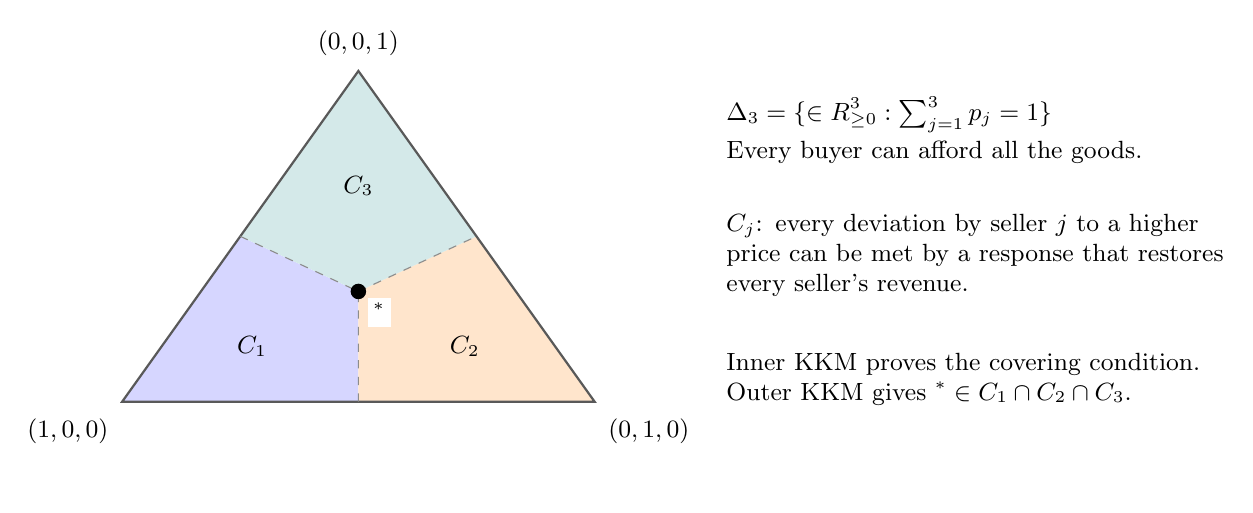
\begin{tikzpicture}[x=1cm,y=1cm,font=\fontsize{9}{10.8}\selectfont]
\path[use as bounding box] (-.2,-.35) rectangle (15,5.45);
\coordinate (v1) at (1.0,.7);\coordinate (v2) at (7.0,.7);\coordinate (v3) at (4.0,4.9);
\coordinate (ps) at (4.0,2.10);
\fill[blue!16] (v1)--(4,.7)--(ps)--(2.5,2.8)--cycle;
\fill[orange!20] (v2)--(5.5,2.8)--(ps)--(4,.7)--cycle;
\fill[teal!17] (v3)--(2.5,2.8)--(ps)--(5.5,2.8)--cycle;
\draw[black!65,line width=.8pt] (v1)--(v2)--(v3)--cycle;
\draw[black!45,dashed] (4,.7)--(ps)--(2.5,2.8);
\draw[black!45,dashed] (ps)--(5.5,2.8);
\node at (2.65,1.4) {$C_1$};\node at (5.35,1.4) {$C_2$};\node at (4,3.44) {$C_3$};
\fill[black] (ps) circle (2.8pt);
\node[anchor=north west,fill=white,inner sep=2pt] at (4.11,2.03) {$\pvec^*$};
\node[anchor=north east] at (.95,.61) {$(1,0,0)$};
\node[anchor=north west] at (7.05,.61) {$(0,1,0)$};
\node[anchor=south] at (4,4.97) {$(0,0,1)$};
\node[anchor=west,text width=6.4cm,align=left] at (8.55,4.15)
 {$\displaystyle\Delta_3 = \{\pvec \in \mathbb{R}_{\ge 0}^3: \textstyle\sum_{j=1}^3 p_j = 1\}$\\[3pt]Every buyer can afford all the goods.};
\node[anchor=west,text width=6.4cm,align=left] at (8.55,2.56)
 {$C_j$: every deviation by seller $j$ to a higher price can be met by a response that restores every seller's revenue.};
\node[anchor=west,text width=6.4cm,align=left] at (8.55,.99)
 {Inner KKM proves the covering condition.\\Outer KKM gives $\pvec^* \in C_1 \cap C_2 \cap C_3$.};
\end{tikzpicture}

\caption{A schematic KKM cover of $\Delta_3$ for three sellers.
Each face is covered by the labels of its vertices, so some point $\pvec^*$ lies in all three sets.
In the outer KKM, $\pvec \in C_j$ means that every (bounded) deviation by seller $j$ to a higher price
can be met by a response that restores every seller's revenue.}
\label{fig:kkm-simplex}
\end{figure}

\paragraph{Inner KKM: raising prices to restore revenues.}
Fix prices $\pvec \in \Delta_m$, and for simplicity, assume that all prices are positive.
For each seller $j$, pick an arbitrary cap $z_j > p_j$ on her price.
We show that there exist prices $\qvec$ in the box $\prod_{j=1}^m [p_j, z_j]$
such that some seller's price reaches her cap, i.e., $q_i = z_i$ for some seller $i$,
and every seller gets her original revenue back, i.e., $R(\qvec) = n\pvec$
(\cref{thm:prop-box}; see \cref{fig:kkm-box}).
However, we cannot control which seller's price reaches her cap.

For any direction $\theta \in \Delta_m$, we raise the prices from $\pvec$ in direction $\theta$
until some seller's price reaches her cap, i.e., we go to the point
\[ y(\theta) \defeq \pvec + \tau(\theta)\theta, \quad \text{where} \quad
    \tau(\theta) \defeq \bigg(\max_{j \in [m]} \frac{\theta_j}{z_j - p_j}\bigg)^{-1}. \]
The map $y$ is continuous.
Label $\theta$ with $j$ if $R_j(y(\theta)) \ge np_j$, i.e., if seller $j$ gets her original revenue back.
(Note that here we label directions, which is different from labeling prices as above.)
Since the allocation rule is continuous, the label sets are closed.
To check the covering condition, let $\theta$ lie on the $S$-face of $\Delta_m$.
Then every seller outside $S$ keeps her old price, so she earns at most her old revenue.
If every seller in $S$ also earned less than her old revenue,
then the total revenue at $y(\theta)$ would be less than $n$.
But since $y(\theta) \ge \pvec$, the sum of prices at $y(\theta)$ is at least 1,
so by strict monotonicity of utilities, every buyer spends her entire budget,
and the total revenue is exactly $n$.
Hence, $\theta$ has some label from $S$.
By KKM, some direction $\theta$ has all labels, i.e., $R_j(y(\theta)) \ge np_j$ for every seller $j$.
Since the entries of both $R(y(\theta))$ and $n\pvec$ sum to $n$,
we get $R(y(\theta)) = n\pvec$.

\begin{figure}[t]
\centering
\begin{tikzpicture}[x=1cm,y=1cm,font=\fontsize{9}{10.8}\selectfont,
  ray/.style={draw=blue!55!black,line width=.65pt},
  axis/.style={-{Stealth[length=2mm]},draw=black!65}]
\path[use as bounding box] (-.2,-.3) rectangle (15,5.4);
\coordinate (p) at (1.05,.72);
\fill[blue!4] (p) rectangle (7.1,4.7);
\draw[black!60] (p) rectangle (7.1,4.7);
\draw[axis] (.7,.42)--(7.55,.42) node[right] {$q_1$};
\draw[axis] (.7,.42)--(.7,5.03) node[above] {$q_2$};
\foreach \x/\y in {7.1/1.7,7.1/2.8,7.1/3.8,6.2/4.7,4.6/4.7,2.8/4.7} {\draw[ray] (p)--(\x,\y);}
\draw[blue!65!black,line width=1.1pt] (p)--(7.1,3.8);
\fill[orange!75!black] (7.1,3.8) circle (2.5pt);
\node[anchor=west,fill=white,inner sep=2pt] at (7.26,3.8) {$y(\theta)$};
\fill[black] (p) circle (2.4pt);
\node[anchor=north west] at (1.03,.64) {$\pvec = (0.5, 0.5)$};
\node[anchor=south east] at (7.1,5.09) {$\zvec = (0.95, 0.9)$};
\draw[blue!60!black,-{Stealth[length=2mm]}] (2.2,1.68) arc[start angle=42,end angle=70,radius=1.55];
\node[fill=white,inner sep=1pt] at (2.6,2.09) {$\theta$};
\fill[teal!70!black] (4.6,4.7) circle (2.5pt);
\node[anchor=south,fill=white,inner sep=1pt] at (3.75,4.79) {$\qvec$: revenues restored};
\node[anchor=west,text width=6.1cm,align=left] at (8.82,4.15)
 {\textbf{Choose a direction $\theta$.}\\Raise prices from $\pvec$ in direction $\theta$ until some seller's price reaches her cap.};
\node[anchor=west,text width=6.1cm,align=left] at (8.82,2.53)
 {\textbf{Label by revenue.}\\Label $\theta$ with $j$ if $R_j(y(\theta)) \ge np_j$.};
\node[anchor=west,text width=6.1cm,align=left] at (8.82,.87)
 {\textbf{Intersect the labels.}\\KKM gives $\qvec$ with $R(\qvec) = n\pvec$, where some seller's price is at her cap.};
\end{tikzpicture}

\caption{The inner KKM for two sellers.
We fix prices $\pvec$ and caps $\zvec$, and raise the prices from $\pvec$ in different directions $\theta$
until they reach the upper boundary of the box $\prod_{j=1}^m [p_j, z_j]$.
KKM gives a direction in which every seller's revenue is restored,
and some seller's price is at her cap.
The marked point $\qvec$ is schematic.}
\label{fig:kkm-box}
\end{figure}

\paragraph{Outer KKM: one price vector for all sellers.}
We now apply KKM to the price simplex $\Delta_m$ itself.
We only need to consider deviations where each seller $j$'s price is at most some large bound $L_j$
(otherwise good $j$ becomes so expensive that no buyer will spend a non-negligible amount on it
if the other goods can exhaust her budget, making the deviation pointless),
and we will find responses where each responder $k$'s price is at most $L_k$.
Formally, let $C_j$ be the set of prices $\pvec \in \Delta_m$ that are labeled by seller $j$, i.e.,
for every deviation $q_j \in [p_j, L_j]$ by seller $j$,
there is a response $\qvec_{-j} \in \prod_{k \ne j} [p_k, L_k]$ such that $R(\qvec) = n\pvec$.
Then any point in $\bigcap_{j=1}^m C_j$ satisfies \cref{eq:overview-restoration} for bounded deviations.
The definition of $C_j$ has both universal and existential quantifiers,
so the main step is to prove the covering condition.

Let $\pvec \in \Delta_m$, let $S$ be the set of sellers with positive prices,
and suppose $\pvec \notin C_j$ for every $j \in S$.
Then each seller $j \in S$ has a \emph{bad deviation} $z_j \in (p_j, L_j]$
for which no response restores every seller's revenue.
Use these bad deviations as caps in the inner KKM (sellers outside $S$ keep their price 0).
It gives prices $\qvec$ with $R(\qvec) = n\pvec$, where $q_i = z_i$ for some seller $i \in S$.
But then $\qvec_{-i}$ is a response to seller $i$'s bad deviation that restores every seller's revenue,
which is a contradiction.
Hence, $\pvec$ has some label from $S$, so the covering condition holds.
The label sets are closed, since the bounded responses lie in a compact set
and the allocation rule is continuous.
Thus, KKM gives us prices $\pvec^* \in \bigcap_{j=1}^m C_j$ (\cref{thm:rare-exists-continuous-2}).
These ideas form the core of \cref{thm:rare-exists-continuous}.

\subsection{Dynamics}
\label{sec:overview:dynamics}

Recall from \cref{sec:intro:results} that prices $\pvec$ form a RARE,
up to an arbitrarily small additive error,
iff $R_j(\pvec) \ge V_j(\pvec_{-j})$ for every seller $j$.
Also recall that in our dynamic, all prices are initially 0,
and in each round, some of the sellers $j$ for which $p_j < V_j(\pvec_{-j})/n$
raise their price to $V_j(\pvec_{-j})/n$.

The key to the analysis is the price vector $\pvec^* \in \Delta_m$
that satisfies \cref{eq:overview-restoration}, which acts as a ceiling for the dynamic
(see \cref{fig:dynamics-path}).
Specifically, for any prices $\pvec \le \pvec^*$ (coordinatewise) and any seller $j$,
we have $V_j(\pvec_{-j}) \le np^*_j$ (\cref{thm:vbound-pstar}).
To see this, suppose seller $j$ deviates to price $q_j$ at prices $\pvec$.
If $q_j \le p^*_j$, then her revenue is at most $nq_j \le np^*_j$, irrespective of any response.
Otherwise, use the response $\qvec_{-j}$ that restores every seller's revenue
when seller $j$ makes the same deviation at prices $\pvec^*$.
Each responder $k$'s revenue at $\qvec$ is then $np^*_k$.
This is at least $np_k$, which in turn is at least $R_k((q_j, \pvec_{-j}))$.
So $\qvec_{-j}$ is also an IR response at prices $\pvec$,
and it limits the deviator's revenue to $np^*_j$.
(Here we use the stronger property in \cref{eq:overview-restoration},
i.e., that responders get back their revenue from before the deviation.)

\begin{figure}[t]
\centering
\begin{tikzpicture}[x=1cm,y=.9cm,font=\fontsize{9}{10.8}\selectfont,
  dynstep/.style={draw=blue!65!black,line width=1.2pt,-{Stealth[length=2mm]}}]
\path[use as bounding box] (-.2,-.4) rectangle (15,5.5);
\coordinate (o) at (1,.6);
\coordinate (pstar) at (4.6,2.6);
\fill[black!3] (o)--(7,.6)--(1,5.6)--cycle;
\fill[blue!8] (o) rectangle (pstar);
\draw[black!55] (1,5.6)--(7,.6);
\draw[blue!55!black,densely dotted,line width=.8pt] (1,2.6)--(pstar)--(4.6,.6);
\draw[-{Stealth[length=2mm]},black!65] (.75,.6)--(7.35,.6) node[right] {$p_1$};
\draw[-{Stealth[length=2mm]},black!65] (1,.35)--(1,5.72) node[above] {$p_2$};
\node[anchor=north] at (1,.5) {$0$};
\draw[dynstep] (o)--(2.2,.6);
\draw[dynstep] (2.2,.6)--(2.2,1.4);
\draw[dynstep] (2.2,1.4)--(3.25,1.4);
\draw[dynstep] (3.25,1.4)--(3.25,1.82);
\fill[blue!65!black] (3.25,1.82) circle (2.5pt);
\node[anchor=south east,fill=white,inner sep=2pt] at (3.14,1.98) {May stop here};
\fill[black] (pstar) circle (2.8pt);
\node[anchor=south west,fill=white,inner sep=2pt] at (4.68,2.63) {$\pvec^* = (0.6, 0.4)$};
\node[rotate=-40,fill=white,inner sep=1pt] at (2.7,4.23) {$p_1 + p_2 = 1$};
\node[anchor=west,text width=6.3cm,align=left] at (8.7,4.4)
 {\textbf{Invariant}\quad $\vecZero \le \pvec^{(t)} \le \pvec^*$\\The prices never exceed $\pvec^*$.};
\node[anchor=west,text width=6.3cm,align=left] at (8.7,2.69)
 {\textbf{Potential}\quad $\sum_{j=1}^m p_j$\\The sum of prices never decreases and is at most 1.};
\end{tikzpicture}

\caption{A possible path of our dynamic for two sellers,
where $\pvec^{(t)}$ denotes the prices after round $t$.
The prices start at $\vecZero$ and never exceed $\pvec^*$,
so they stay in the shaded box below the line $p_1 + p_2 = 1$,
and the sum of prices never decreases.
In this path, the sellers raise their prices one at a time.
The dynamic may stop at prices other than $\pvec^*$.}
\label{fig:dynamics-path}
\end{figure}

By induction, the prices never exceed $\pvec^*$.
In particular, the sum of prices is always at most 1,
so every buyer buys every good completely, and each seller $j$'s revenue is always $np_j$.
Hence, the sum of prices is a potential function that never decreases and is at most 1.
After round $t$, let $g_t$ be the largest amount by which some seller $j$'s $V_j(\pvec_{-j})$
exceeds her revenue $R_j(\pvec)$ (or 0 if there is no such seller).
Then the prices after round $t$ are a $\delta$-additive RARE for every $\delta > g_t$.
If the most unsatisfied seller raises her price in round $t+1$,
then the sum of prices increases by at least $g_t/n$.
Hence, $\sum_{t \ge 0} g_t \le n = B$.
So $g_t < \delta$ for some $t \le \floor{B/\delta}$,
and $g_t \ge \delta$ for at most $\floor{B/\delta}$ values of $t$.
This gives us \cref{thm:dynamics-convergence}.

\paragraph{Organization.}
\Cref{sec:prelims} formally defines our model and RARE.
\Cref{sec:revenue-props} states some properties of the revenue function, and a way to unify the analysis of the rivalrous and the non-rivalrous settings.
\Cref{sec:exist} proves the existence of RARE, and \cref{sec:dynamics} analyzes our dynamic.
\Cref{sec:exist-extra} contains the proofs omitted from \cref{sec:exist}.
\Cref{sec:lim-rare-equiv} proves \cref{thm:rare-equiv-defn}, i.e.,
the relationship between $V_j$ and RARE.
\Cref{sec:nasheq-uncommon} shows that Nash equilibria are uncommon.
